\documentclass[11pt,english]{article}
\usepackage{babel}
\usepackage{verbatim}
\usepackage{float}
\usepackage{amsmath}
\usepackage{amssymb}
\usepackage[left=2.7cm,right=2.7cm,top=2.7cm,bottom=2.7cm]{geometry}
\usepackage{graphicx}
\usepackage{subcaption}

\setlength{\parindent}{0pt}
\newcommand{\reffig}[1]{Figure \ref{#1}\hspace{2pt}}


\begin{document}
Kun Zhou \hfil UID: 204688165	
	
P1. \\
i) I think step 3 is more efficient than step 2, because with $\sigma_0=1$, the $p(x,y)$ is very small when $\pi(x,y)$ is large.  So It is hard for step 2 to get sample with more useful information.

\begin{figure}[H]
	\includegraphics[height=5in, width=0.8\textwidth]{p1_1.pdf}
	\caption{$\hat{\theta}$ against n} \label{p1_1}
\end{figure}

From \reffig{p1_1}, we can see $\hat{\theta}_1$ of step 1 quickly converges to 4 after sampling amount increase to $10^5$.  For step 2, $\hat{\theta}_2$ are prone to converge to 4, but the estiamted values are not stable even when $N=10^{15}$.  For step 3, $\hat{\theta}_3$ converges to 4 after the amount increases to $10^{10}$.  So step 1 is the best method and step 3 is better than step 2.\\
ii)\\
First calculate the $ess(n)$ for step 2 and step 3.\\
\begin{flalign*}
&\omega = \frac{\pi(x, y)}{p(x,y)}&\\
&E[\omega] = E[\frac{\pi(x, y)}{p(x,y)}] = \int \frac{\pi(x, y)}{p(x,y)}p(x,y) dxdy = 1&\\
&E[\omega^2] = E[\frac{\pi(x, y)^2}{p(x,y)^2}] = \int \frac{\pi(x, y)^2}{p(x,y)}dxdy = \int \frac{\sigma_0^2}{2\pi}e^{-\left[ (x-2)^2+(y-2)^2-\frac{1}{2\sigma_0^2}(x^2+y^2)\right]} dxdy&\\
&= \int \frac{\sigma_0^2}{2\pi} e^{-\left[ (1-\frac{1}{2\sigma_0^2})x^2 - 4x + (1-\frac{1}{2\sigma_0^2})y^2 - 4y + 8 \right]} dxdy&\\
&= \int \frac{\sigma_0^2}{2\pi} e^{-(1-\frac{1}{2\sigma_0^2})\left[x - \frac{4\sigma_0^2}{2\sigma_0^2-1} \right]^2 + \frac{8\sigma_0^2}{2\sigma_0^2-1}}e^{-(1-\frac{1}{2\sigma_0^2})\left[y - \frac{4\sigma_0^2}{2\sigma_0^2-1} \right]^2 + \frac{8\sigma_0^2}{2\sigma_0^2-1}}e^{-8}dxdy&\\
&=\frac{\sigma_0^2}{2\pi}(\sqrt{\frac{\pi}{\frac{2\sigma_0^2-1}{2\sigma_0^2}}})^2e^{\frac{16\sigma_0^2}{2\sigma_0^2-1}}e^{-8}&\\
&=\frac{\sigma_0^4}{2\sigma_0^2-1}e^{\frac{8}{2\sigma_0^2-1}}&\\
&\Rightarrow ess(n) = \frac{n}{1+Var[\omega]} = \frac{n}{E[\omega^2]} = \frac{2\sigma_0^2-1}{\sigma_0^4}e^{\frac{-8}{2\sigma_0^2-1}}n&
\end{flalign*}
For step 2, $\sigma_0=1 \Rightarrow ess(n) = e^{-8}n=0.000335n$.  For step 3, $\sigma_0=4 \Rightarrow ess(n)=0.09355n.$\\
For $ess^{*}$, calculating one $\hat{\theta}$ is not enough to estimate errors, so calculate $\hat{\theta}$ at least 500 times for each step and then calculate the standard deviation of each estimate.  If 2 steps have a similar standard deviation, the estimated errors could be regarded as same.  For example, if $n_1=5$, the standard deviation of step 1 is 0.6282757.  For step 2, $n_2=210000$, the standard deviation of step 2 is 0.5757558.  So we can think $ess^*(n_1) = ess^*(n_2)$ and theoretical value $n_2 = 5 * e^8 = 14904$.
\begin{figure}[H]
	\centering
	\begin{subfigure}[b]{0.475\textwidth}
		\centering
		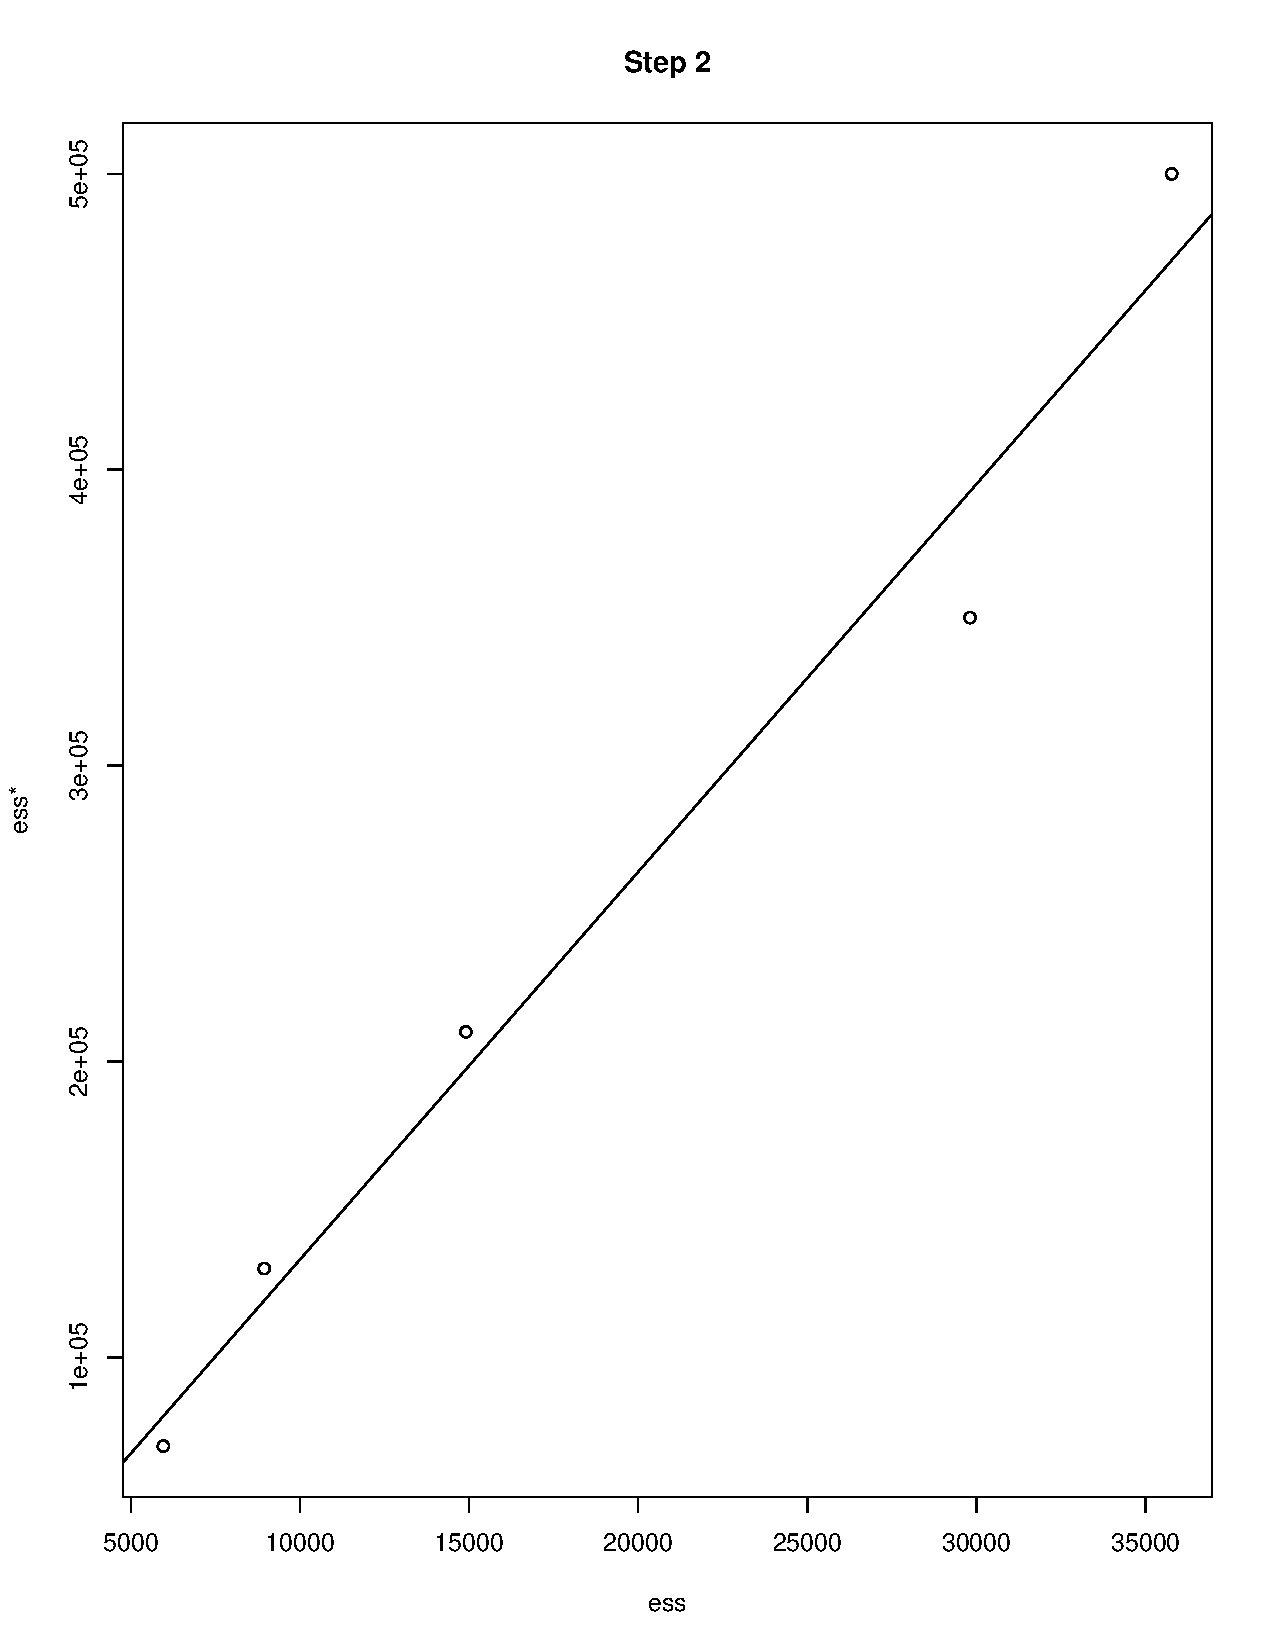
\includegraphics[width=\textwidth, height=6cm]{p1_2.pdf}
		\caption{step 2}\label{p1_2}
	\end{subfigure}
	\quad
	\begin{subfigure}[b]{0.475\textwidth}
		\centering
		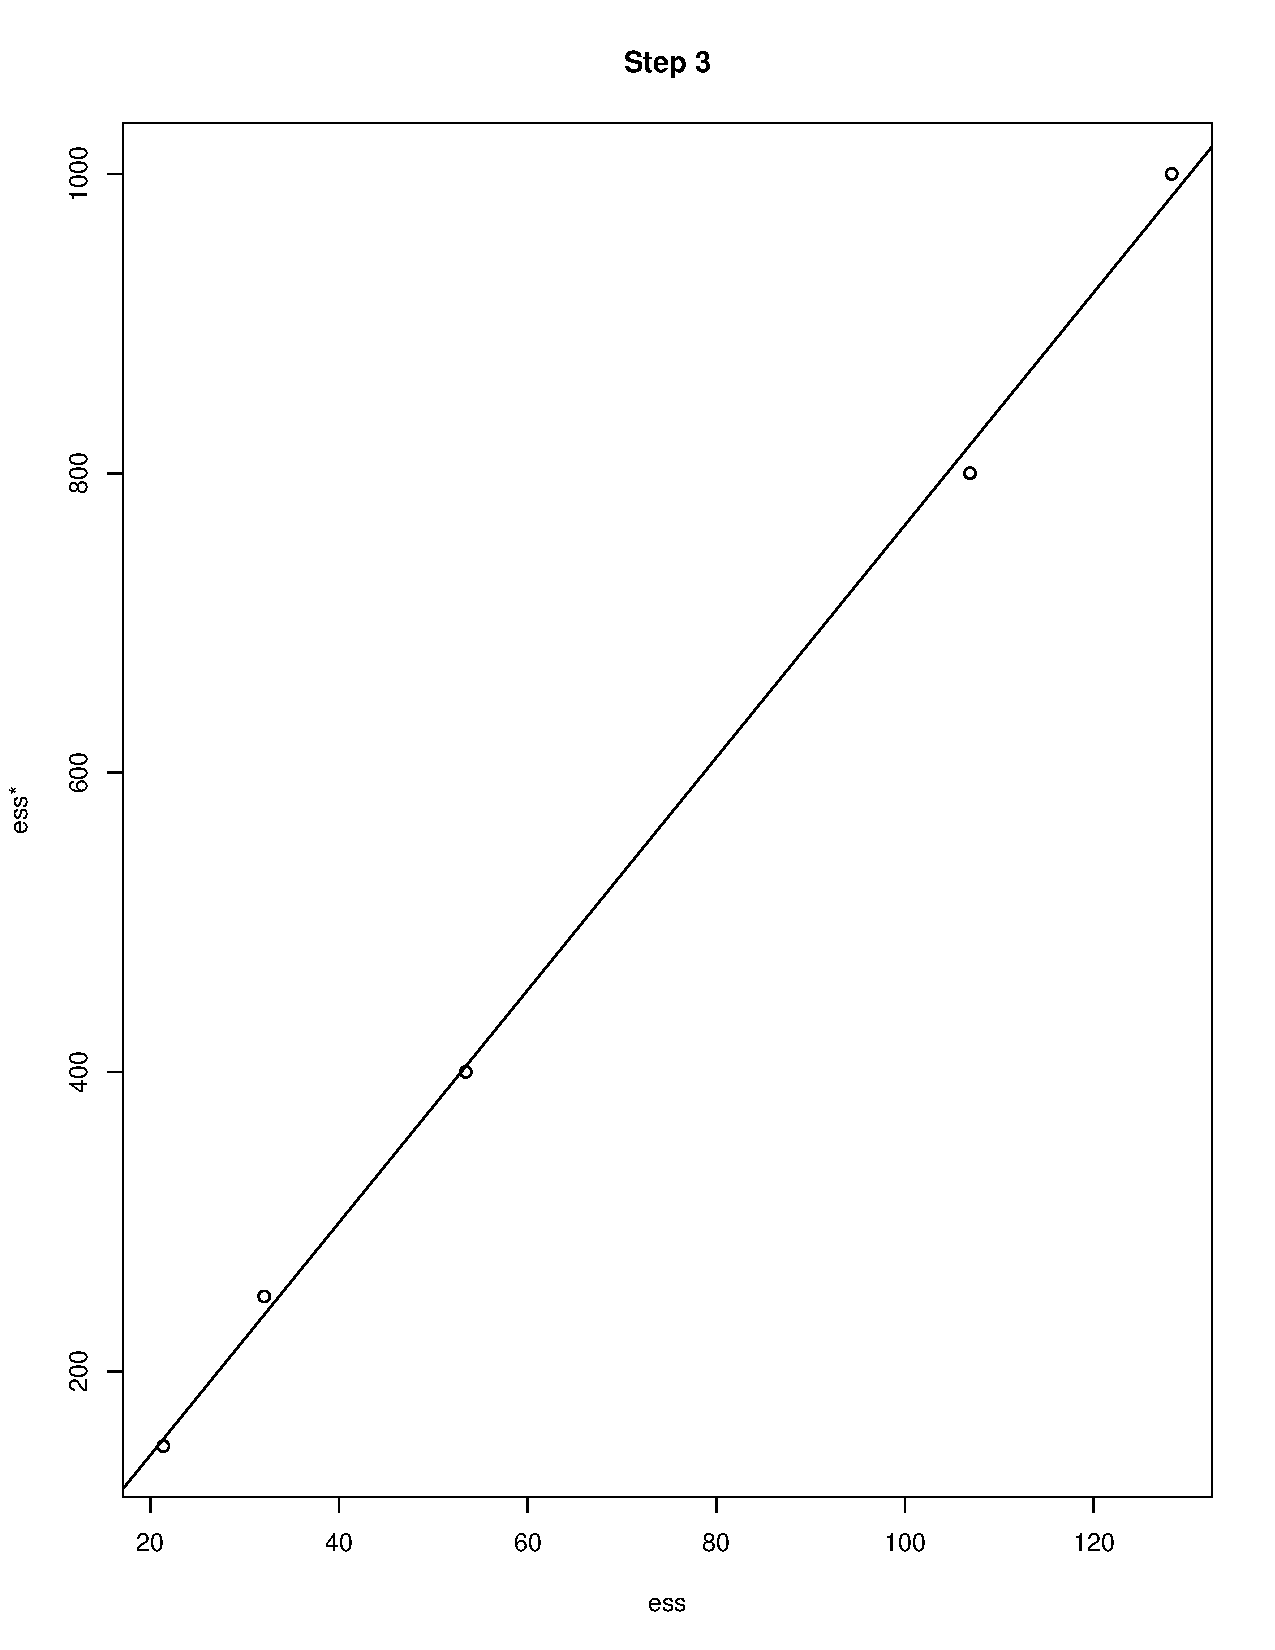
\includegraphics[width=\textwidth, height=6cm]{p1_3.pdf}
		\caption{step 3}\label{p1_3}
	\end{subfigure}
	\caption{}
\end{figure}
We can see $ess$ and $ess^*$ are proportional for both step 2 and step 3.  From \reffig{p1_2} and \reffig{p1_3}, if we want step 2 and step 3 have the same effecive sample size, step 2 requires much more samples.\\
The following is R code.\\


P2.\\
Method 1: I use probability $g_1(x)=\displaystyle\prod_{j=1}^m\frac{1}{k_j}$, where $m$ is the total length of the path, and $k_j$ is the number of possible choices at j-th step.\\
Method 2: I introduce an early termination rate $\epsilon=0.05$ at each step (while in textbook, $\epsilon=0.1$). So $g_2(x) = \displaystyle\prod_{j=1}^m\frac{1}{k_j*0.95}$.\\
Method 3: For any walk that longer than 50, $u=5$ more children based on it are generated and are reweighed by $\omega_0 = \frac{\omega}{u}.$\\
i)\\
\begin{figure}[H]
	\centering
	\begin{subfigure}[b]{0.475\textwidth}
		\centering
		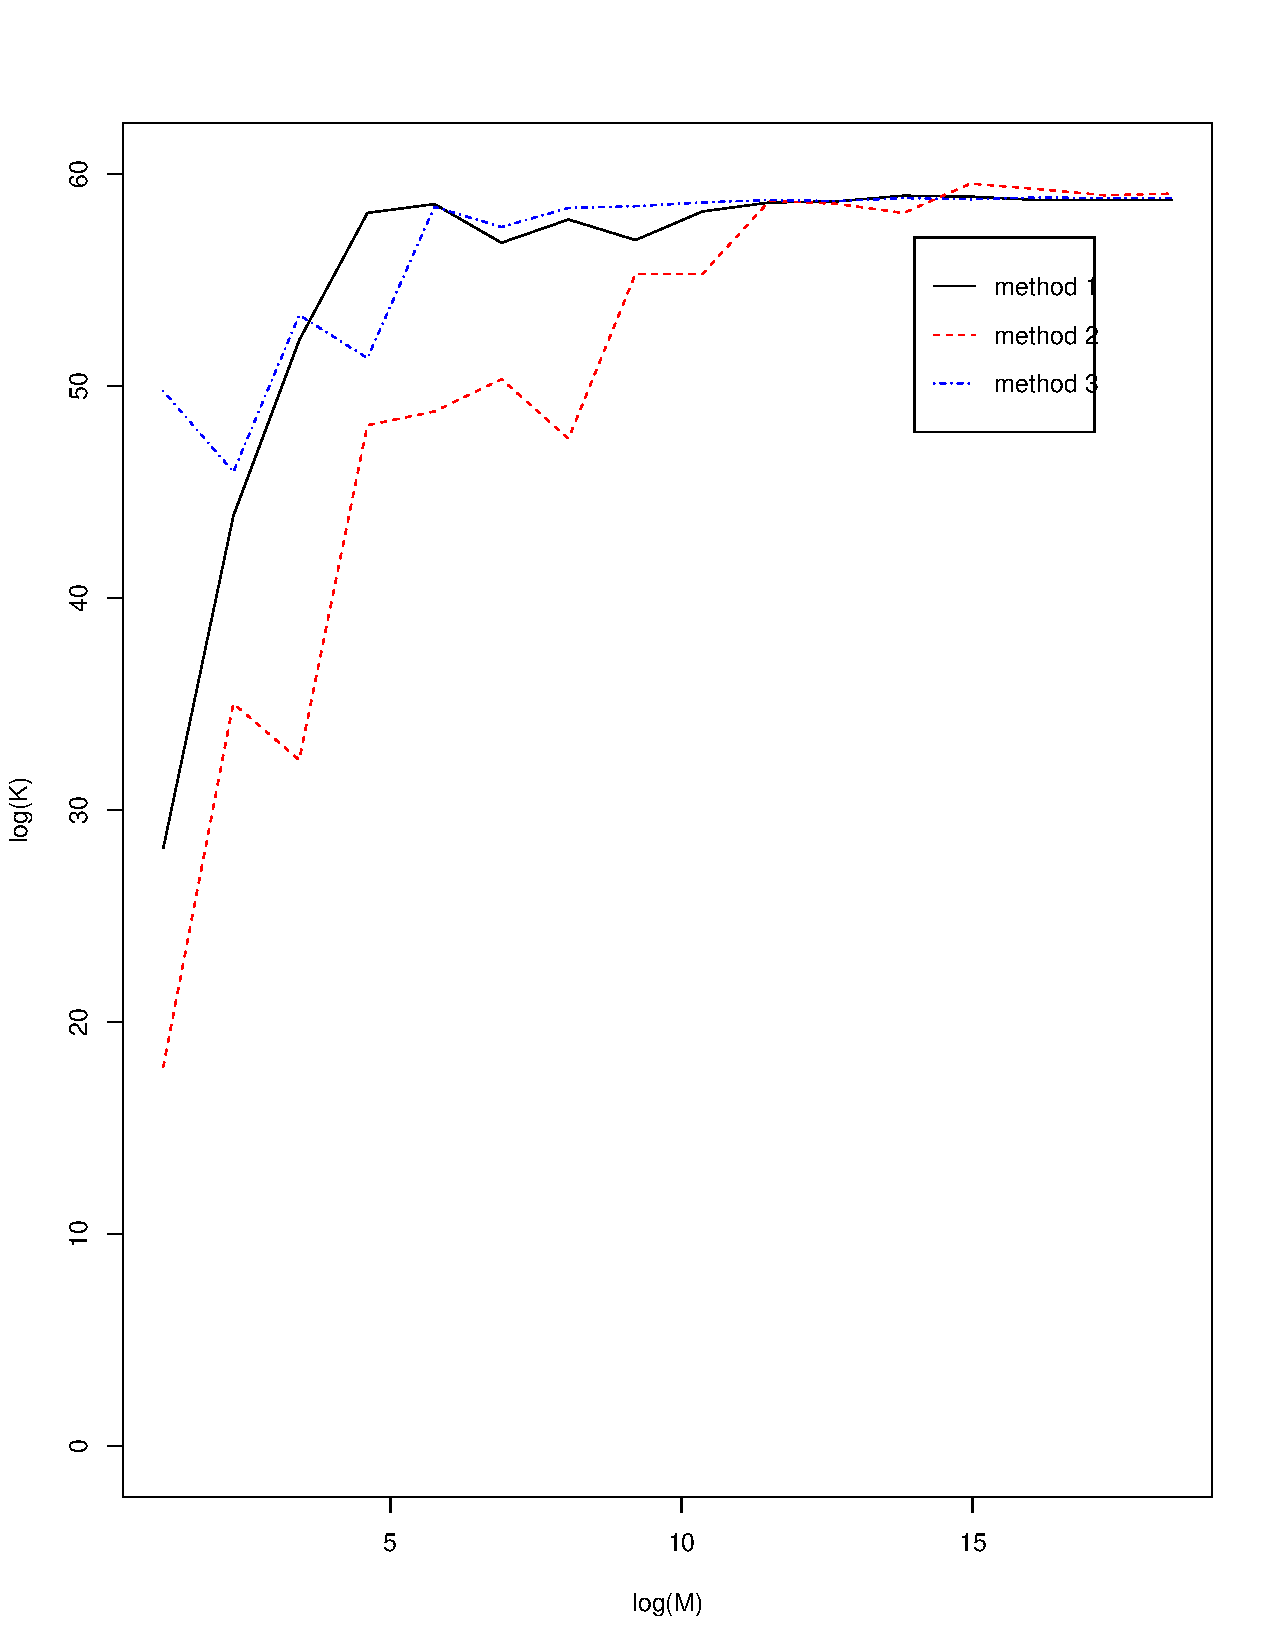
\includegraphics[width=\textwidth, height=6cm]{p2_1_1.pdf}
		\caption{Global log-log plot of K against M}\label{p2_1_1}
	\end{subfigure}
	\quad
	\begin{subfigure}[b]{0.475\textwidth}
		\centering
		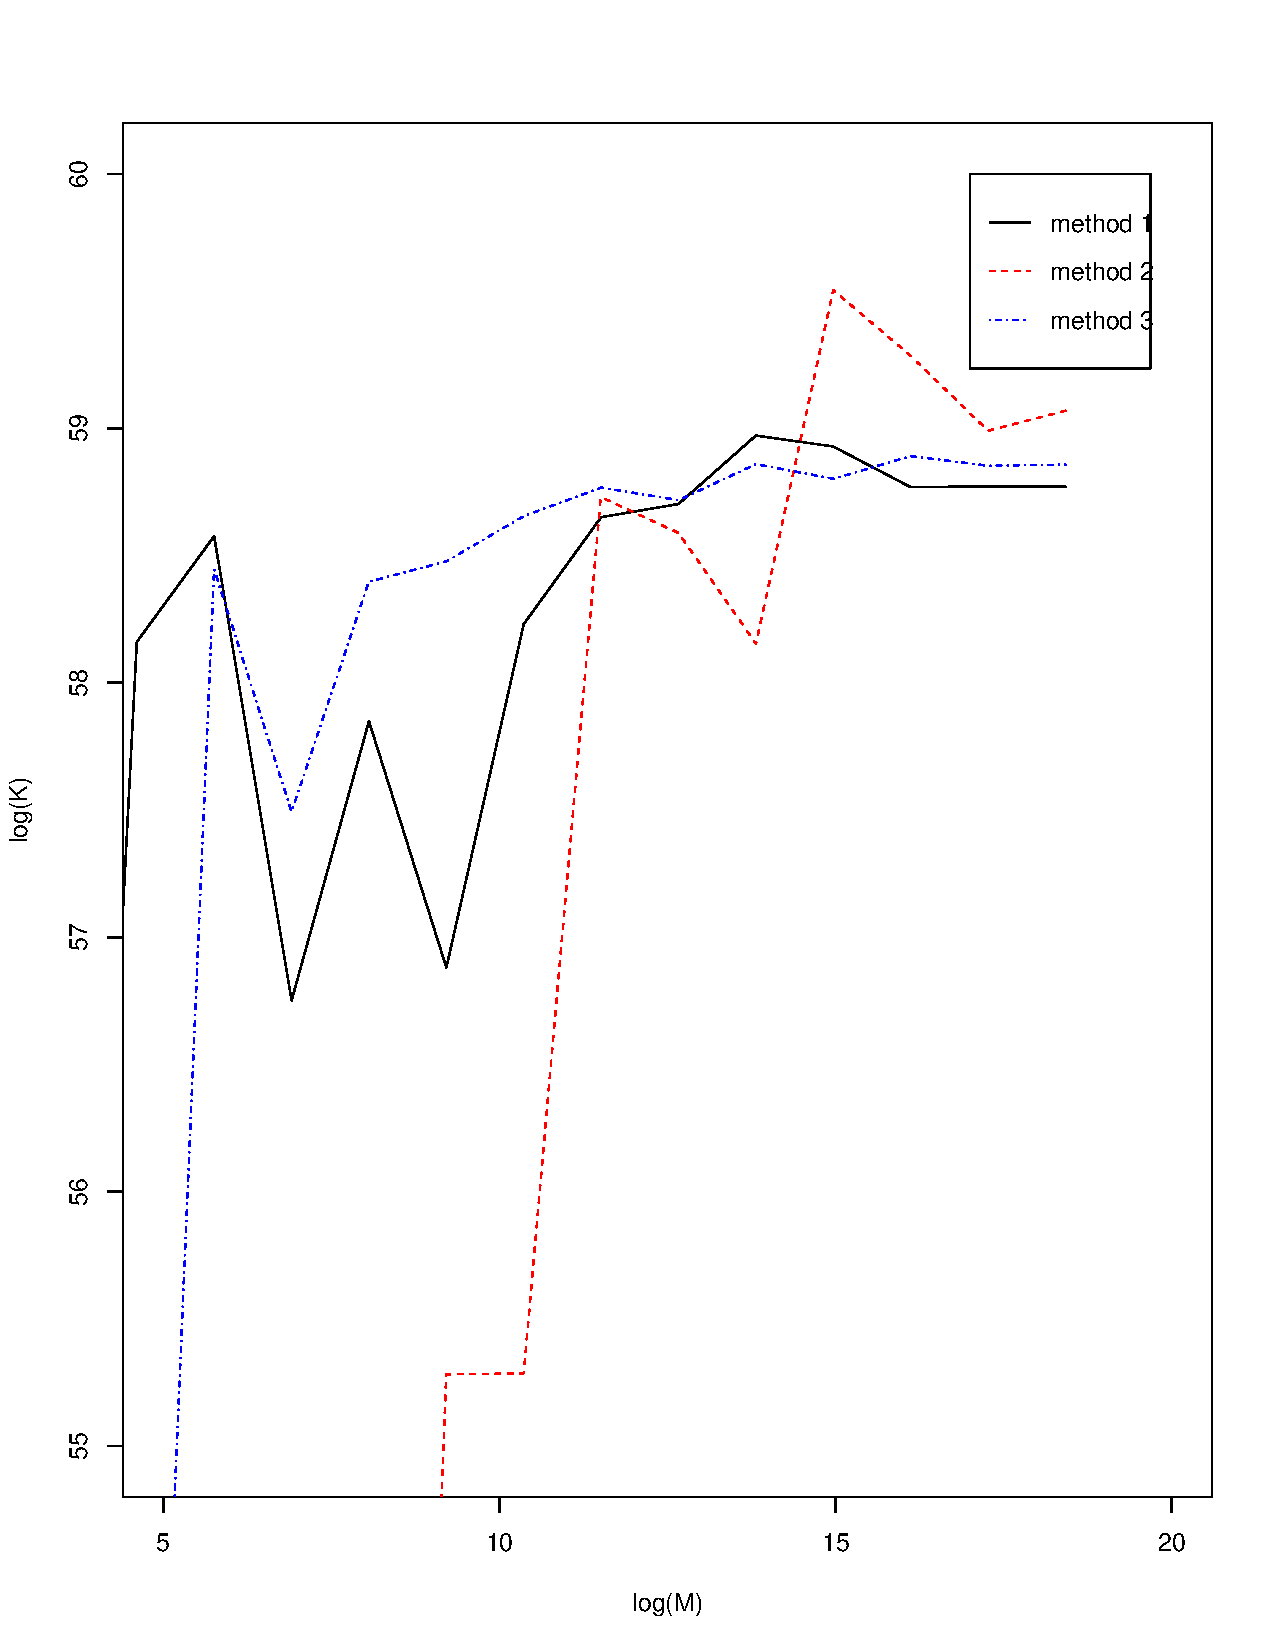
\includegraphics[width=\textwidth, height=6cm]{p2_1_2.pdf}
		\caption{Local log-log plot of K against M}\label{p2_1_2}
	\end{subfigure}
	\caption{}
\end{figure}

From \reffig{p2_1_1}, we can see that SIS processes of all 3 methods are converging with M increasing. \reffig{p2_1_2} demonstrates that Method 3 converges the fastest and Method 2 converges the most slowly. The limit values of Method 2 and Method 3 are higher than Method 1, which means the bias cannot be neglected. The following are the estimated value of $K$s when $M=10^8$ for the 3 methods respectively: $3.316744 * 10^{25}, \quad  4.512596*10^{25}, \quad 3.649155*10^{25}$.\\



ii)\\
I applied the method mentioned in textbook.\\
$1.501552*10^{24}$

iii)
\begin{figure}[H]
	\centering
	\begin{subfigure}[b]{0.475\textwidth}
		\centering
		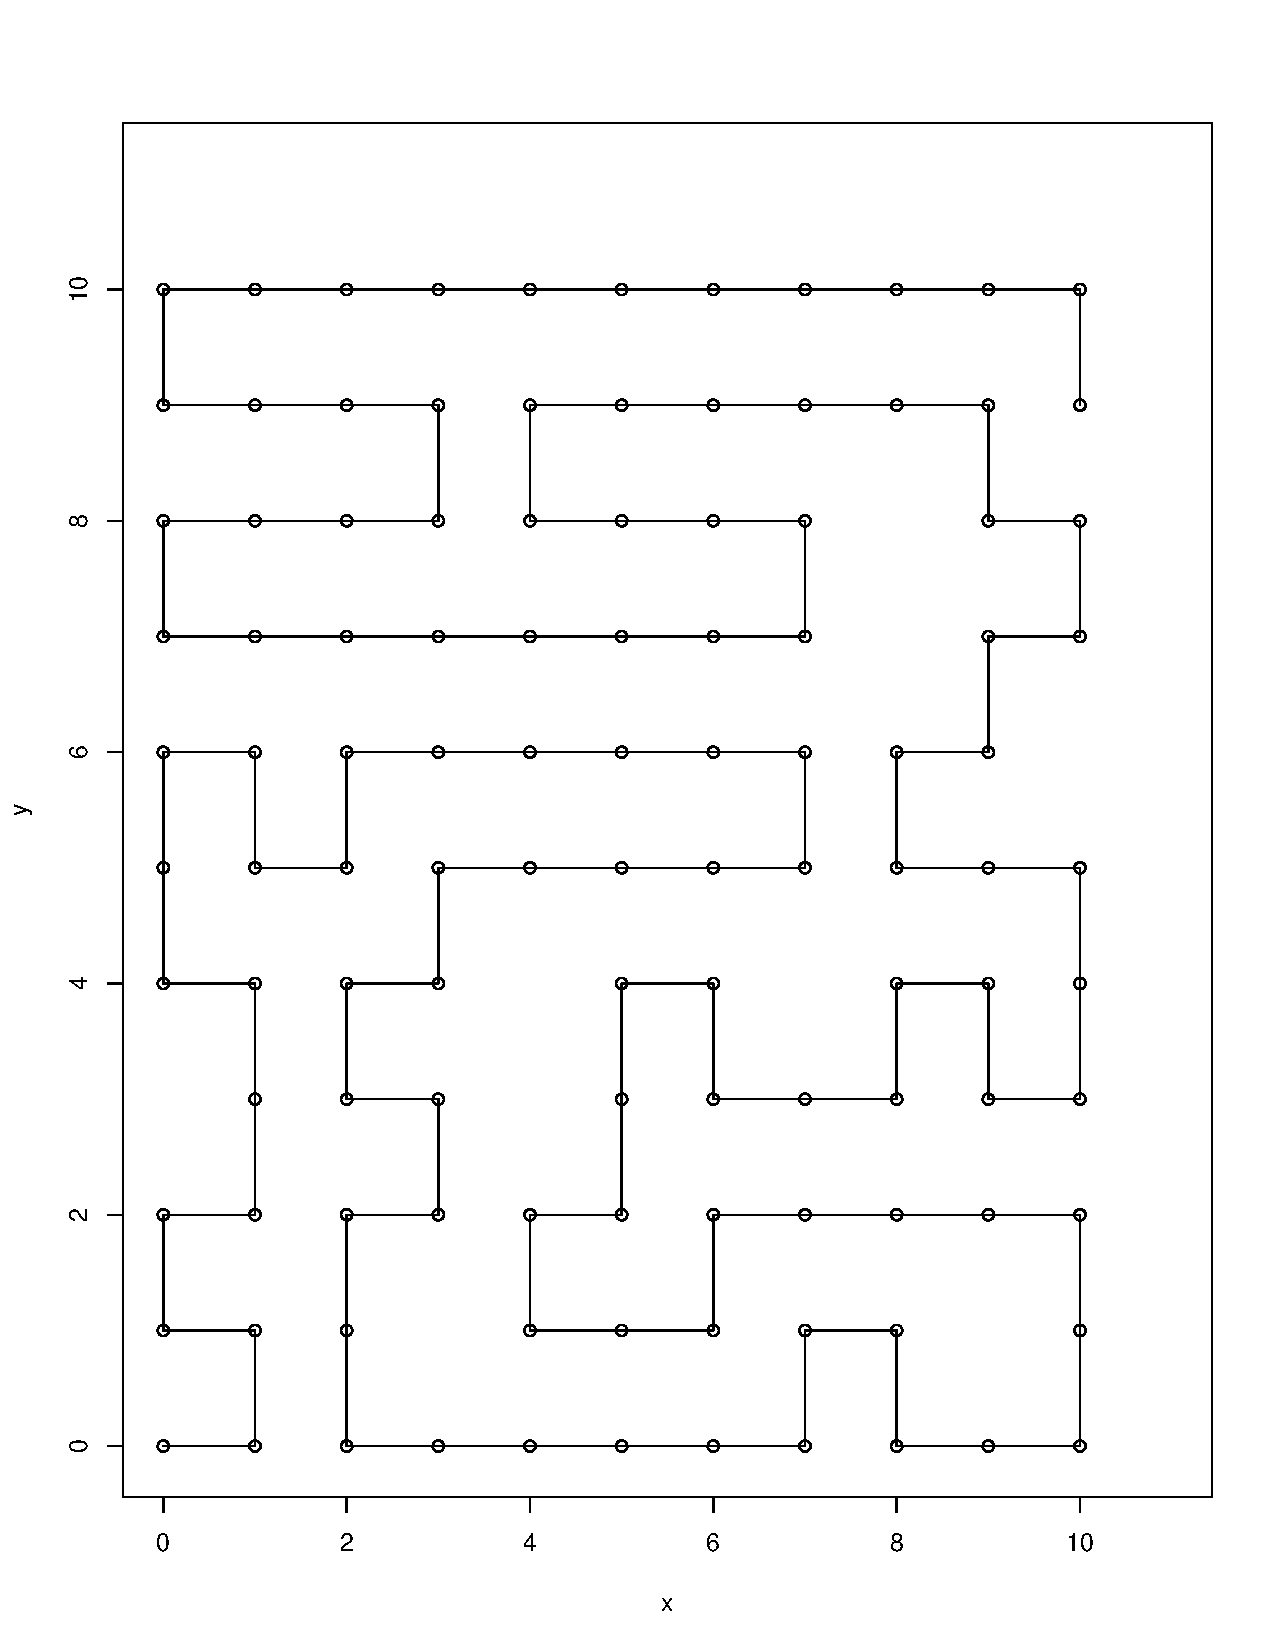
\includegraphics[width=\textwidth, height=6cm]{p2_3_1_111.pdf}
		\caption{Longest path}\label{p2_3_1_111}
	\end{subfigure}
	\quad
	\begin{subfigure}[b]{0.475\textwidth}
		\centering
		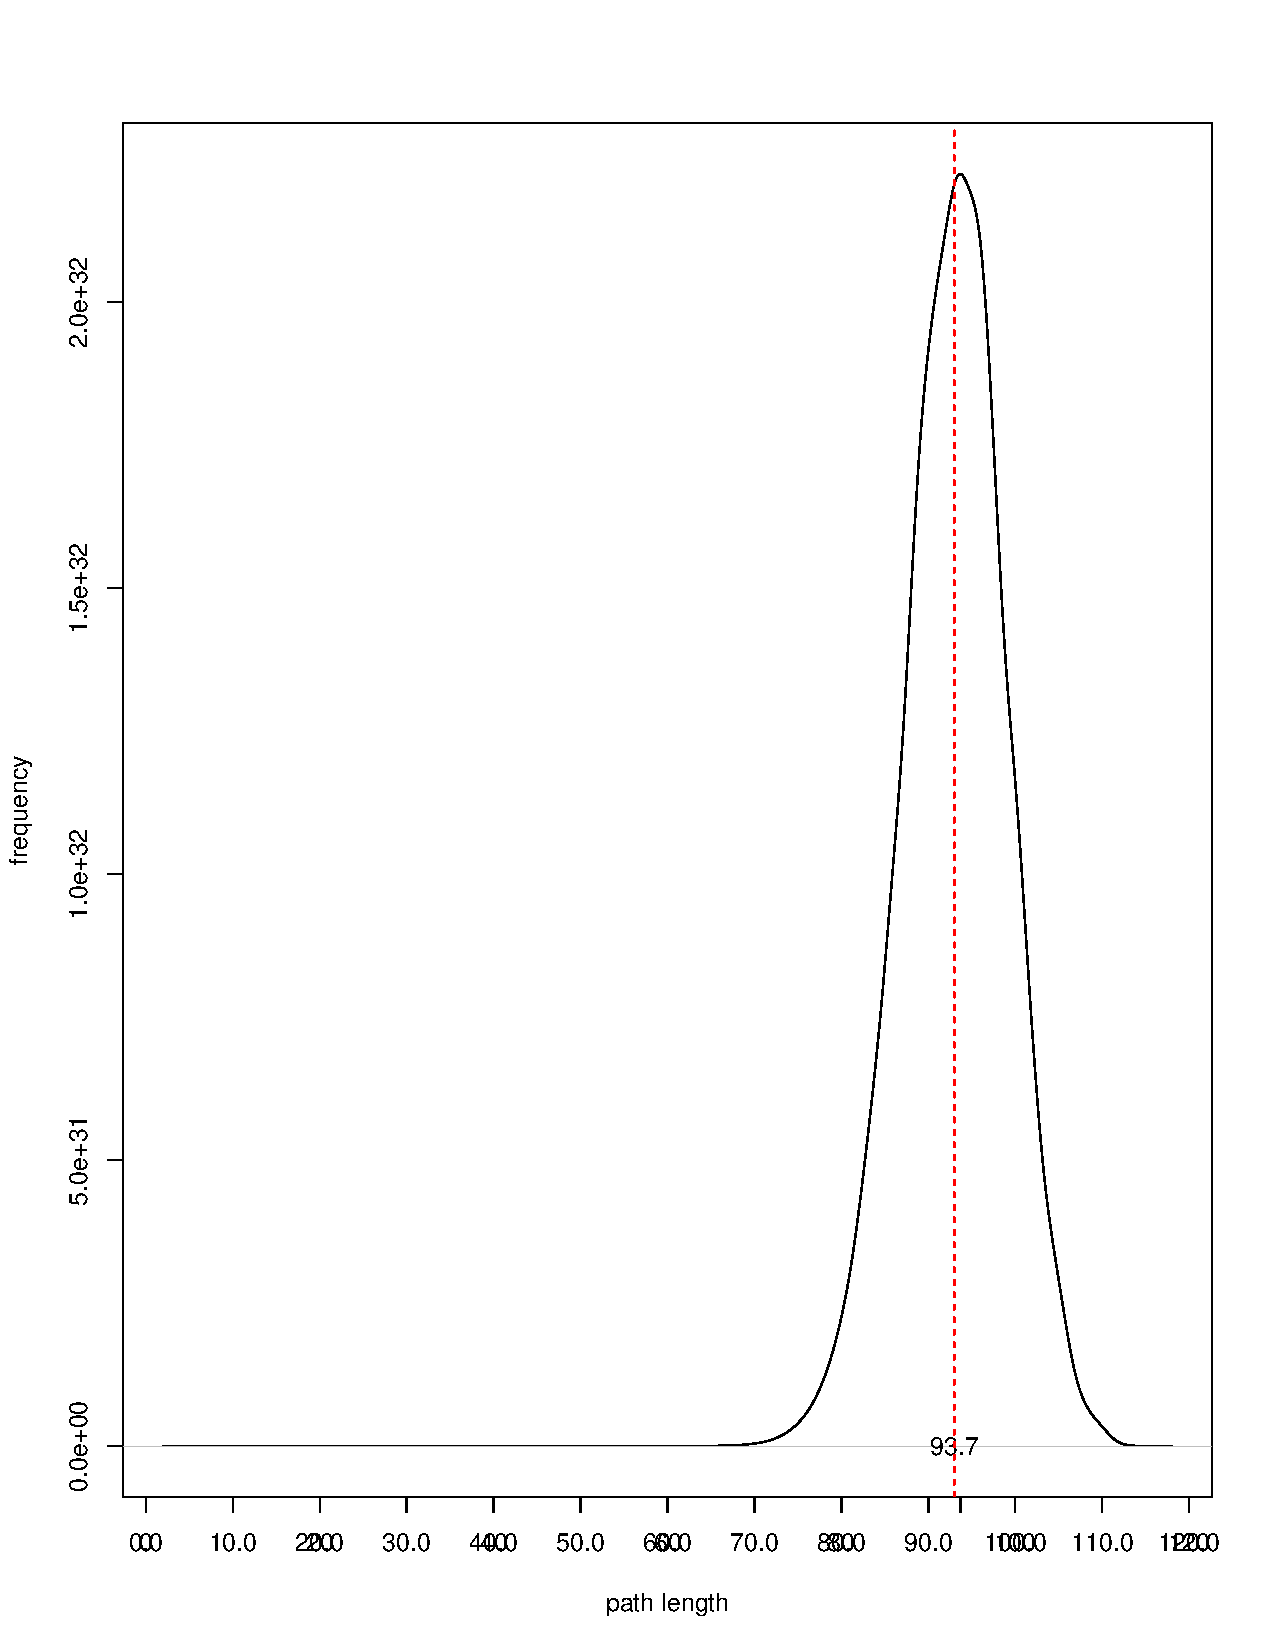
\includegraphics[width=\textwidth, height=6cm]{p2_3_2.pdf}
		\caption{Density function of paths}\label{p2_3_2}
	\end{subfigure}
	\caption{Method 1}
\end{figure}
For Method 1, \reffig{p2_3_1_111} has length 111.  \\
\begin{figure}[H]
	\centering
	\begin{subfigure}[b]{0.475\textwidth}
		\centering
		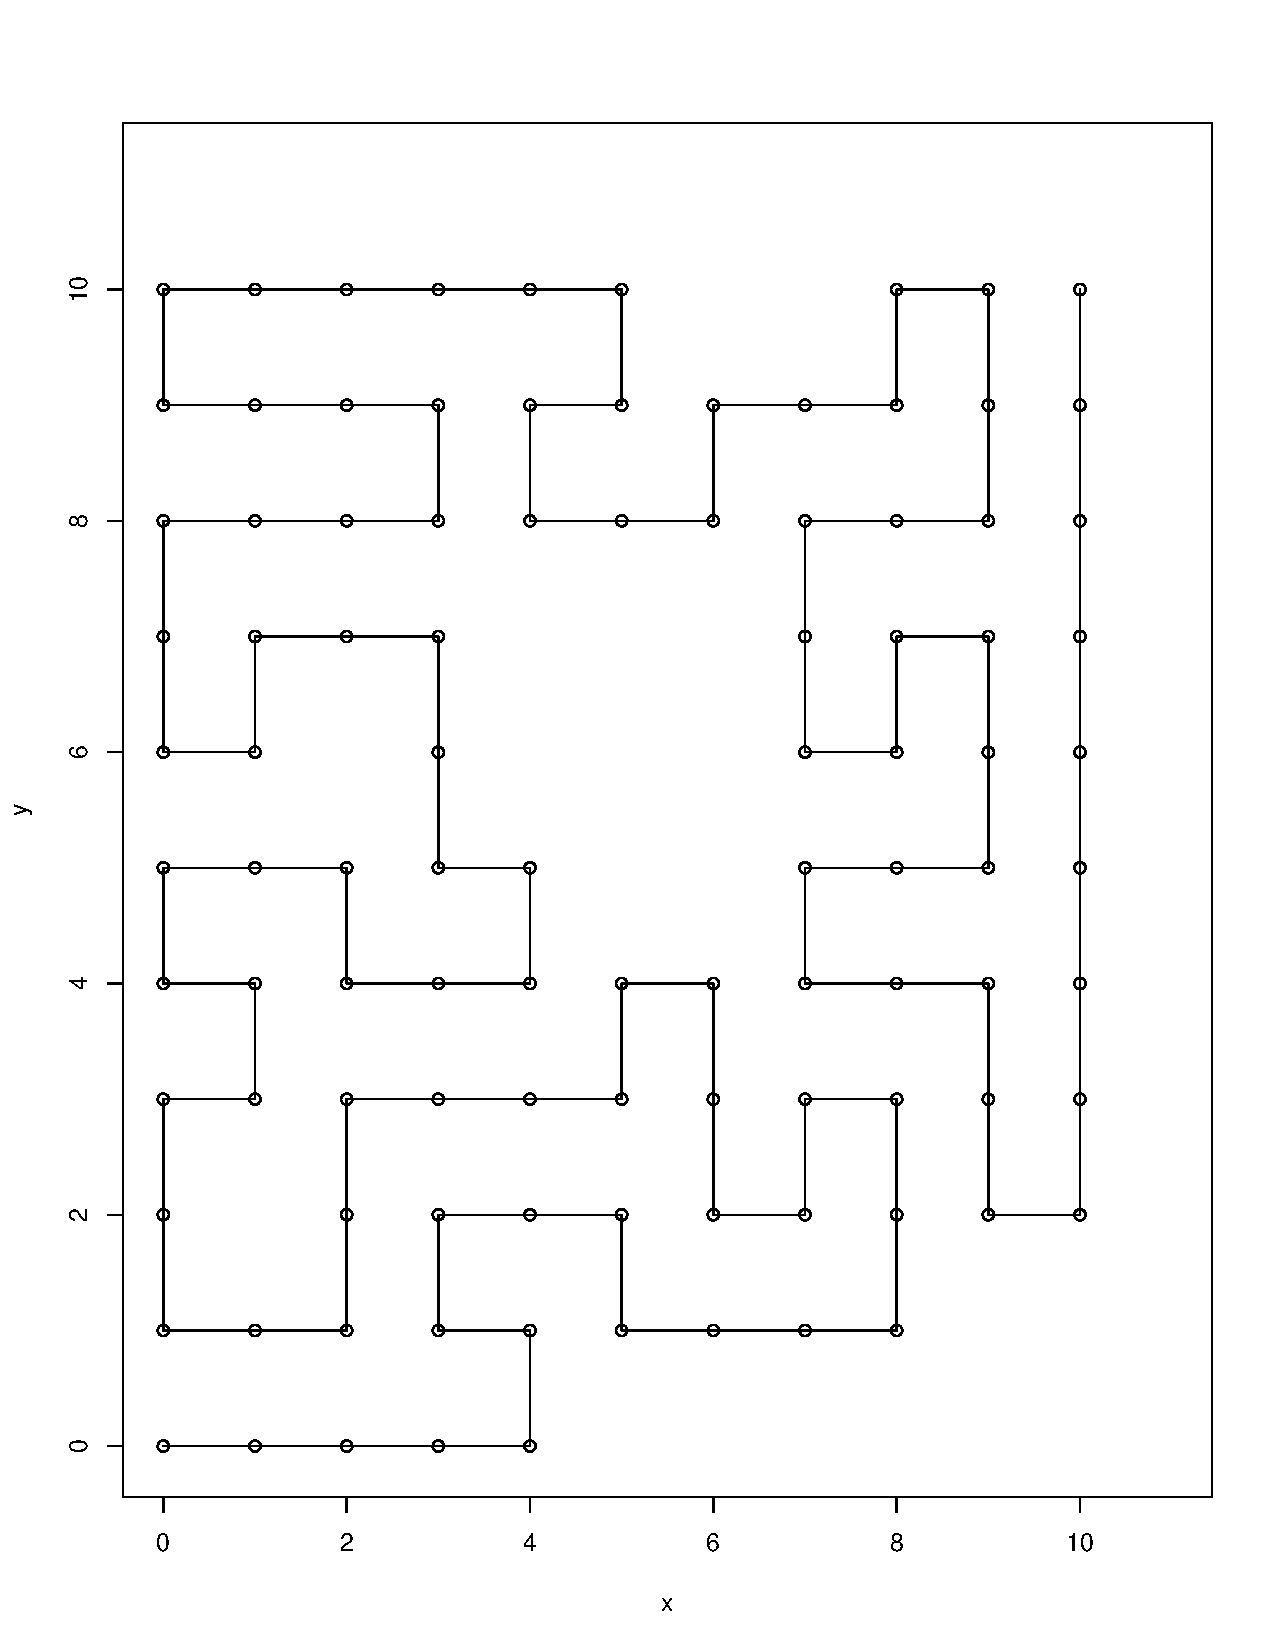
\includegraphics[width=\textwidth, height=6cm]{p2_3_3_100.pdf}
		\caption{Longest path}\label{p2_3_3_100}
	\end{subfigure}
	\quad
	\begin{subfigure}[b]{0.475\textwidth}
		\centering
		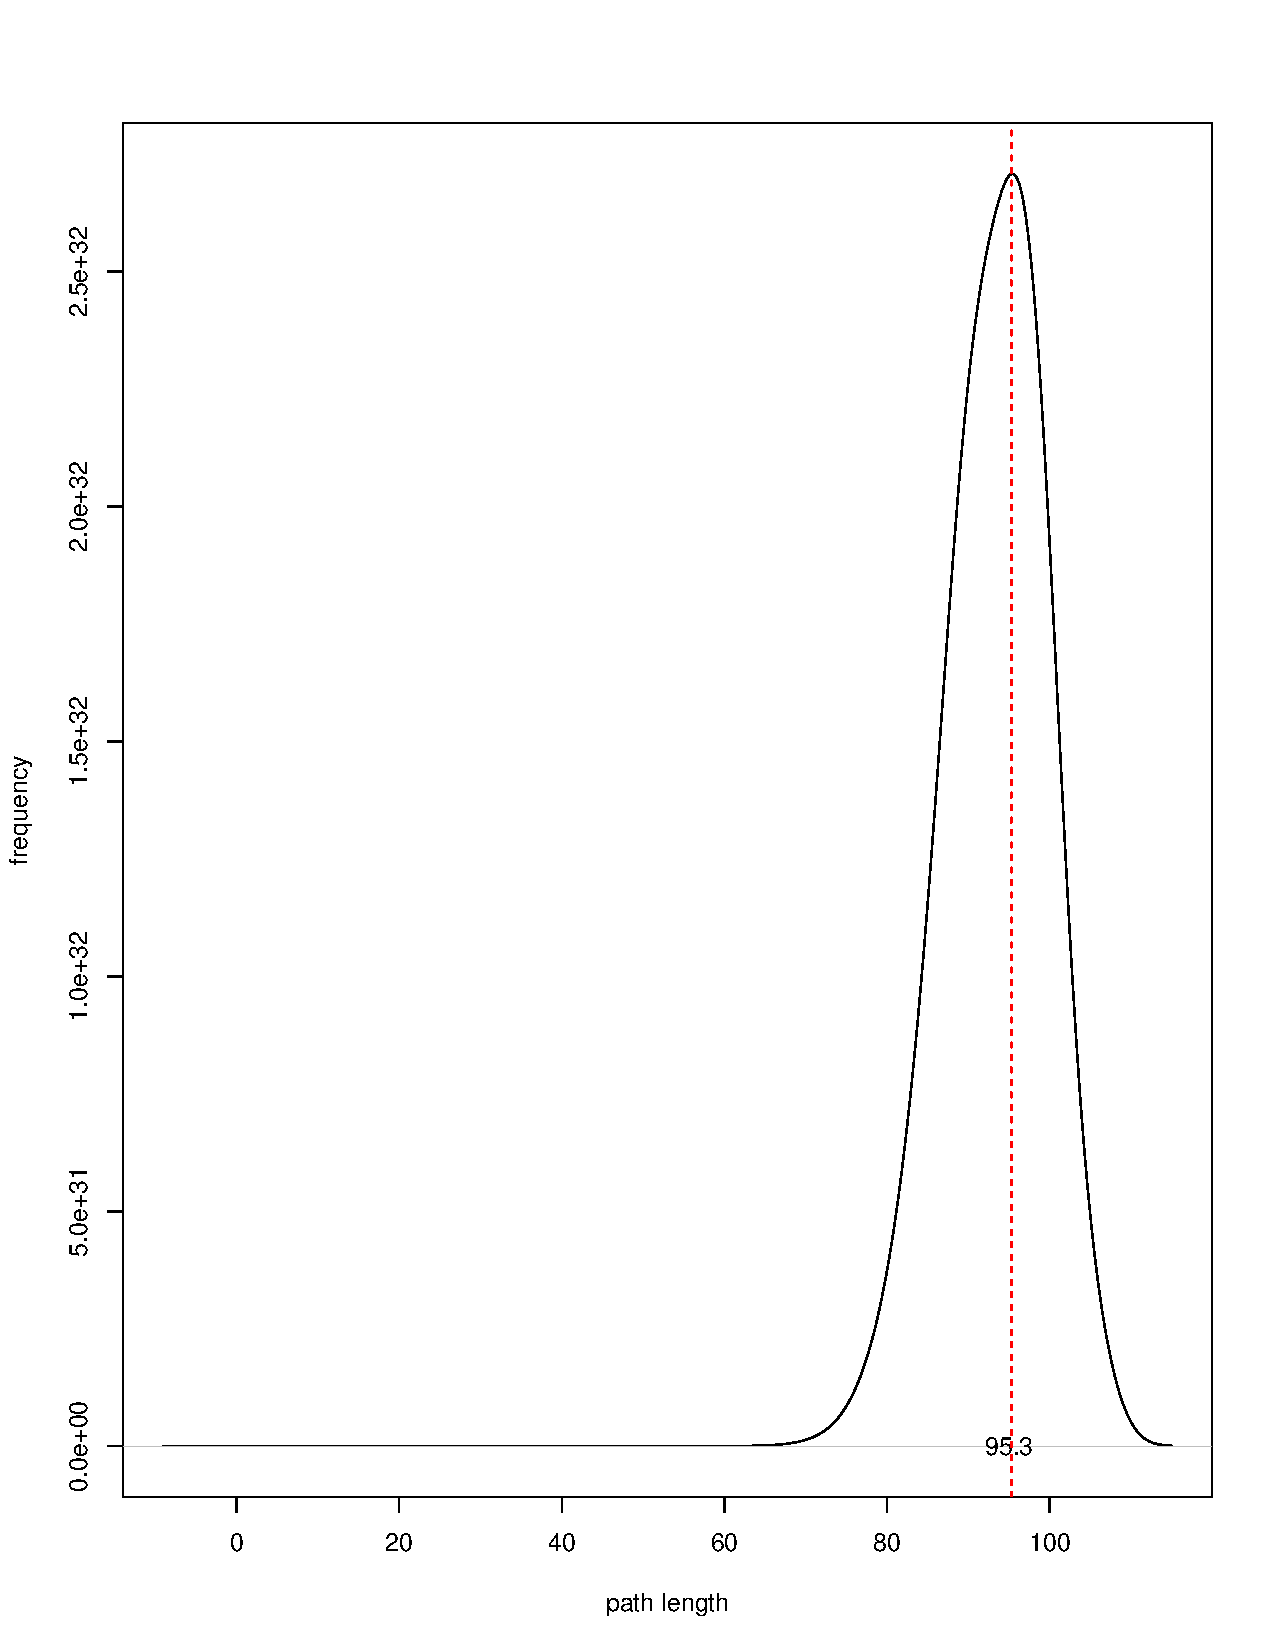
\includegraphics[width=\textwidth, height=6cm]{p2_3_4.pdf}
		\caption{Density function of paths}\label{p2_3_4}
	\end{subfigure}
	\caption{Method 2}
\end{figure}
For Method 2, \reffig{p2_3_3_100} has length 100. \reffig{p2_3_4} is against intuition.  The most dense point is 95.3 while the length of the longest path for Method 2 is 100. But it's reasonable, because $\frac{1}{\epsilon}^m$ makes longer paths' weight much more larger. \\

\begin{figure}[H]
	\centering
	\begin{subfigure}[b]{0.475\textwidth}
		\centering
		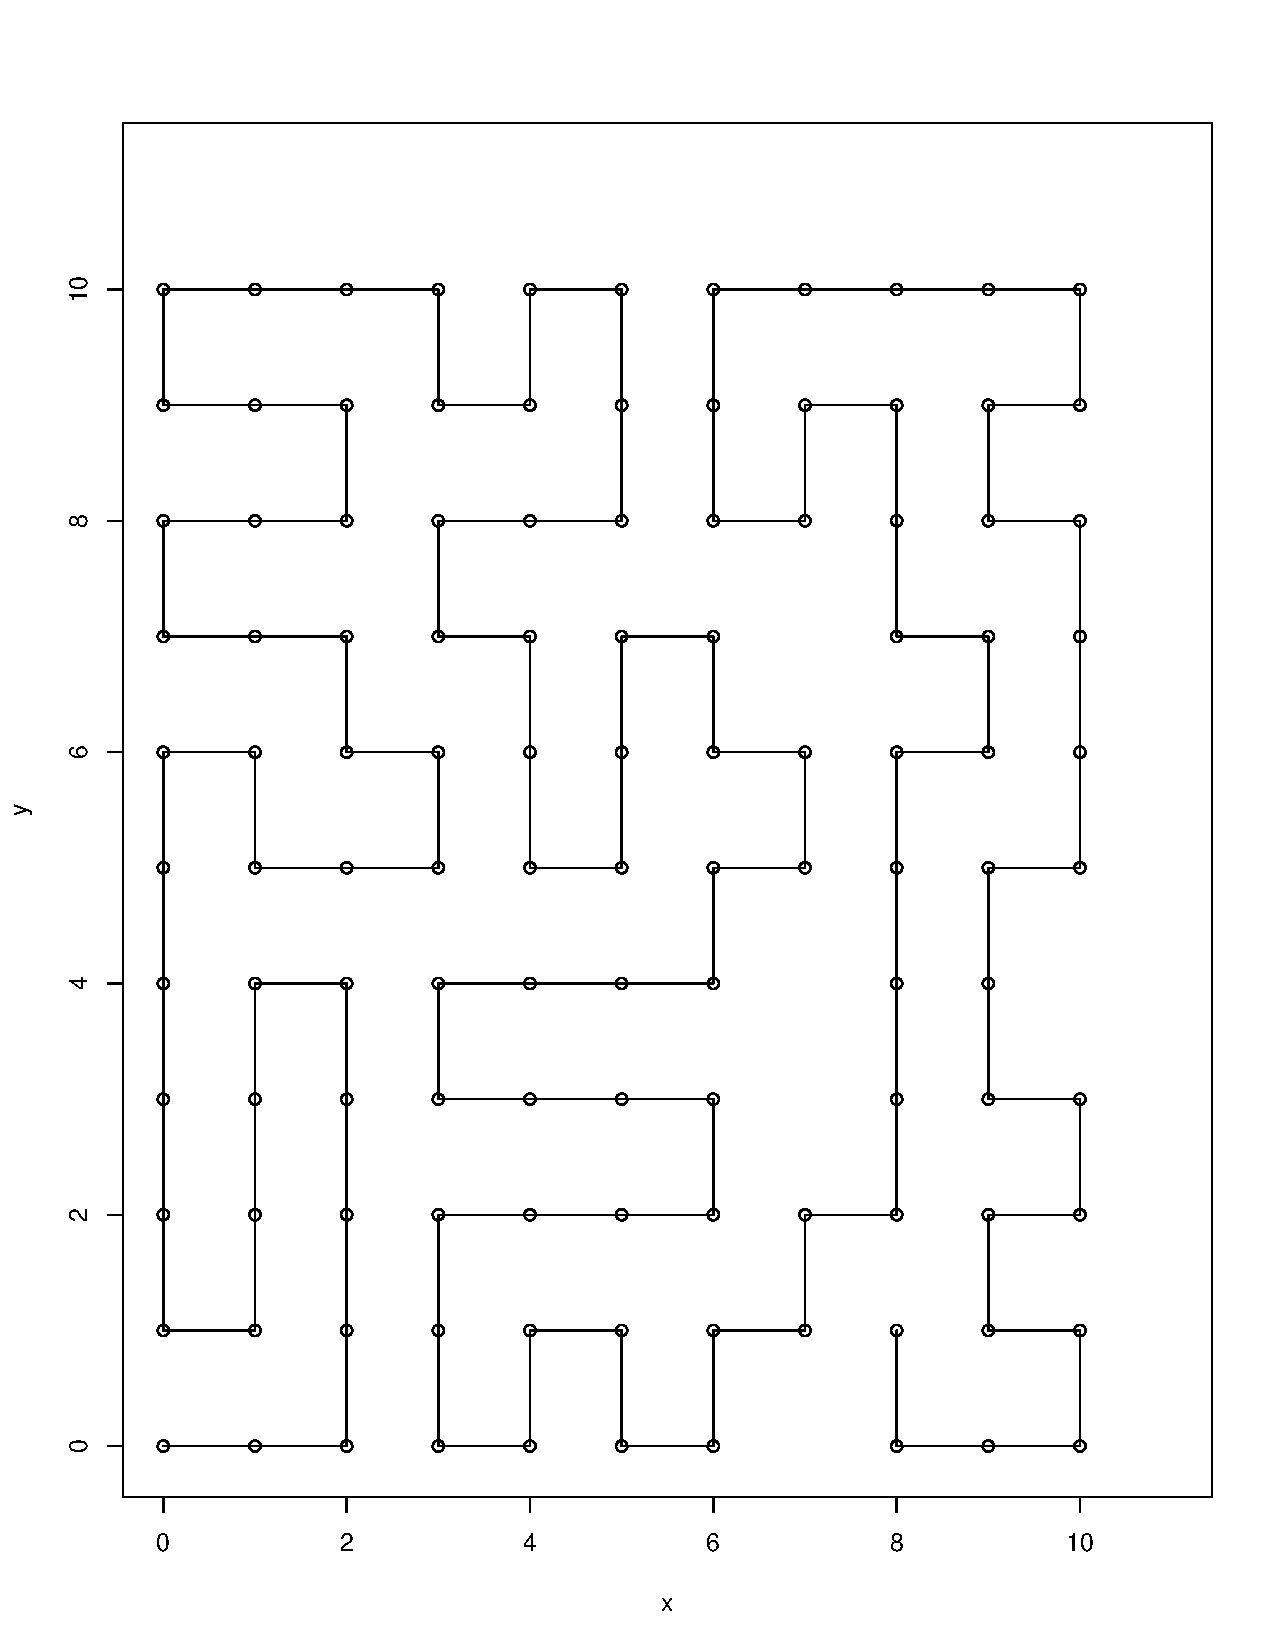
\includegraphics[width=\textwidth, height=6cm]{p2_3_5_115.pdf}
		\caption{Longest path}\label{p2_3_5_115}
	\end{subfigure}
	\quad
	\begin{subfigure}[b]{0.475\textwidth}
		\centering
		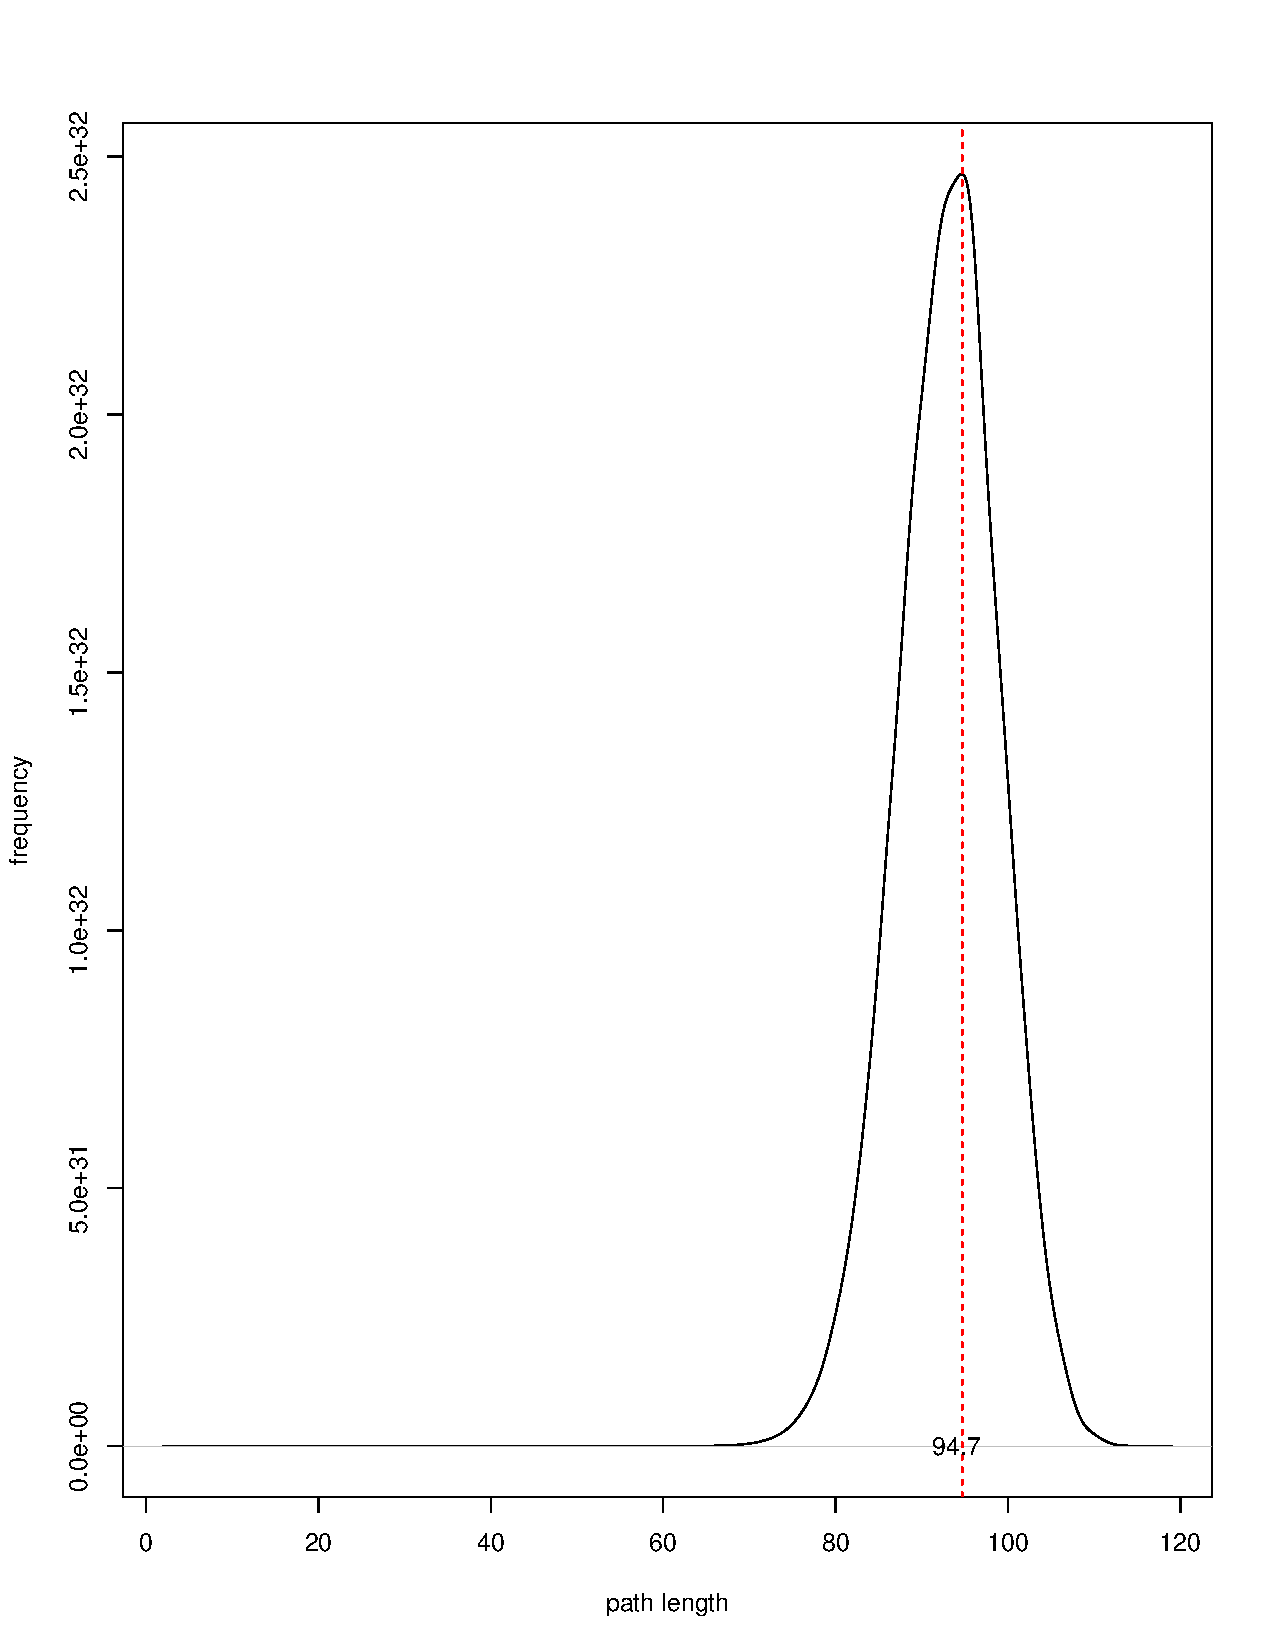
\includegraphics[width=\textwidth, height=6cm]{p2_3_6.pdf}
		\caption{Density function of paths}\label{p2_3_6}
	\end{subfigure}
	\caption{Method 3}
\end{figure}

For Method 3, \reffig{p2_3_5_115} has length 115. The most dense point is 94.7 which is a little higher than the one of Method 1, becuase there are more paths, having length more than 50 and some of which are adapted to new weights.
	
The following are C++ codes for all questions.
	
	
\end{document}
